% estcj.py

\documentclass[10pt,a4paper]{article}
\usepackage[body={16cm,25cm}]{geometry}
\usepackage{hyperref}
\hypersetup{colorlinks=true,linkcolor=blue}
\usepackage{graphicx}
\usepackage{listings}
\lstset{basicstyle=\ttfamily\scriptsize,identifierstyle=,keywordstyle=}
\usepackage{lscape}

%------------------------------------------------------------------
% Extra formatting for codes (from report style)
%------------------------------------------------------------------
% a couple horizontal bars to delimit embedded code
% the width suits that set above and
% the mathmode eliminates spaces between the three elements
\newcommand{\topbar}{\ensuremath{
    \rule{0.1mm}{2.0mm} \rule[2.0mm]{159.5mm}{0.1mm} \rule{0.1mm}{2.0mm}
}}
\newcommand{\bottombar}{\ensuremath{
    \rule{0.1mm}{2.0mm} \rule{159.5mm}{0.1mm} \rule{0.1mm}{2.0mm}
}}

%------------------------------------------------------------------
% Title page information
%------------------------------------------------------------------

\title{
  Estimation of high-enthalpy flow conditions
  for simple shock and expansion processes using
  the ESTCj program and library.
}
\author{
  Mechanical Engineering Report 2011/02 \\
  P.~A.~Jacobs, R.~J.~Gollan, D.~F.~Potter, F.~Zander,\\
  D.~E.~Gildfind, P.~Blyton, W.~Y.~K.~Chan and L.~Doherty \\
  Centre for Hypersonics\\
  The University of Queensland
}

\begin{document}
\maketitle

\baselineskip = 1.2pc

\begin{abstract}
This report presents the software tools that we have built to do simple
flow process calculations for ideal gases and gases in chemical equilibrium.
The software comes in the form of a library for the most fundamental processes and
an application program, ESTCj, for convenient calculation of 
the combined flow processes relevant to shock- and expansion-tube operation.
\end{abstract}

\bigskip
\tableofcontents

%------------------------------------------------------------------

\newpage
\section{Introduction}
%
ESTCj\,\footnote{Equilibrium Shock Tube Conditions, junior} 
began as a re-implementation of the ideas in the ESTC code\,\cite{mcintosh_70}
written by Malcolm McIntosh in the late 1960s and 
the shock-tube-plus-nozzle (STN) code\,\cite{krek_jacobs_93} written in the early 1990s.
The new program\,\cite{jacobs_gardner_2003a} was started 
while PJ was on study leave at DLR Goettingen,
with a decision to delegate the equilibrium thermochemistry issues to the 
Gordon and McBride's Chemical Equilibrium Analysis (CEA) 
code\,\cite{gordon_mcbride_1994,mcbride_gordon_1996}.
With the thermochemistry provided by CEA, the ESTCj program had to be concerned
only with the smaller task of computing the flow changes across shocks and through
the steady nozzle expansion.

\medskip
Implementation was done in the Python programming language\,\footnote{http://www.python.org}
which was easy for end users to customize so the program tended to grow in an ad-hoc fashion.
This report describes the current generation of the program, which has been refactored into
three layers:
\begin{enumerate}
 \item Thermochemical gas models for perfect gases and gases in thermochemical equilibrium.
 \item A library of functions for simple flow processes such as normal shocks, oblique shocks,
  steady and unsteady and expansions.
 \item A top-level code (actually called estcj.py) that coordinates the calling 
  of the flow-process functions using information provided by the user on the command line.
\end{enumerate}
One of the advantages of moving the flow-process calculations to a library is that 
they can be conveniently reused, 
as has been done for the NENZFr code\,\cite{doherty_etal_2012a}, for example.
Two simple examples of building specific programs with the library are shown in
Section\,\ref{custom-apps}.

\medskip
The following sections provide an overview of the new functions and their capabilities.
The bulk of the detail is in the source code which we've tried to make modular and very readable.
Despite the code being central to this report, we put it in the Appendix so that there is
a reasonable chance that the reader might at least get the overview 
before being overwhelmed by detail and giving up.

\newpage
\section{Operation of the ESTCj program}
%
The application-level code is essentially a command-line interpreter
that writes the results of the requested calculation to the standard-output stream
by default.
It's easiest to get a reminder of the available settings by asking for ``help''
on the command line.

\medskip
\noindent\topbar
\lstinputlisting[language={},breaklines=true]{../notes/estcj-help.txt}
\bottombar

The list of available gas models presented as options on the command line is small
and reflects the typical needs of the UQ shock tunnel operation.
The supporting gas model library (Appendix~\ref{cea2-gas-py}) 
calls upon the NASA Glenn CEA2 program 
for evaluation of the equilibrium thermochemical properties 
and it is easy to add entries for other gas mixtures.

\bigskip
\subsection{Example of use for T4 condition}
%
Built into ESTCj is an idealized model of a reflected shock tube.
This model is composed of quasi-one-dimensional wave processes 
as shown in the following figure that has been taken from Ref.\,\cite{krek_jacobs_93}.
The numbers denote states of the gases between processes.

\begin{center}
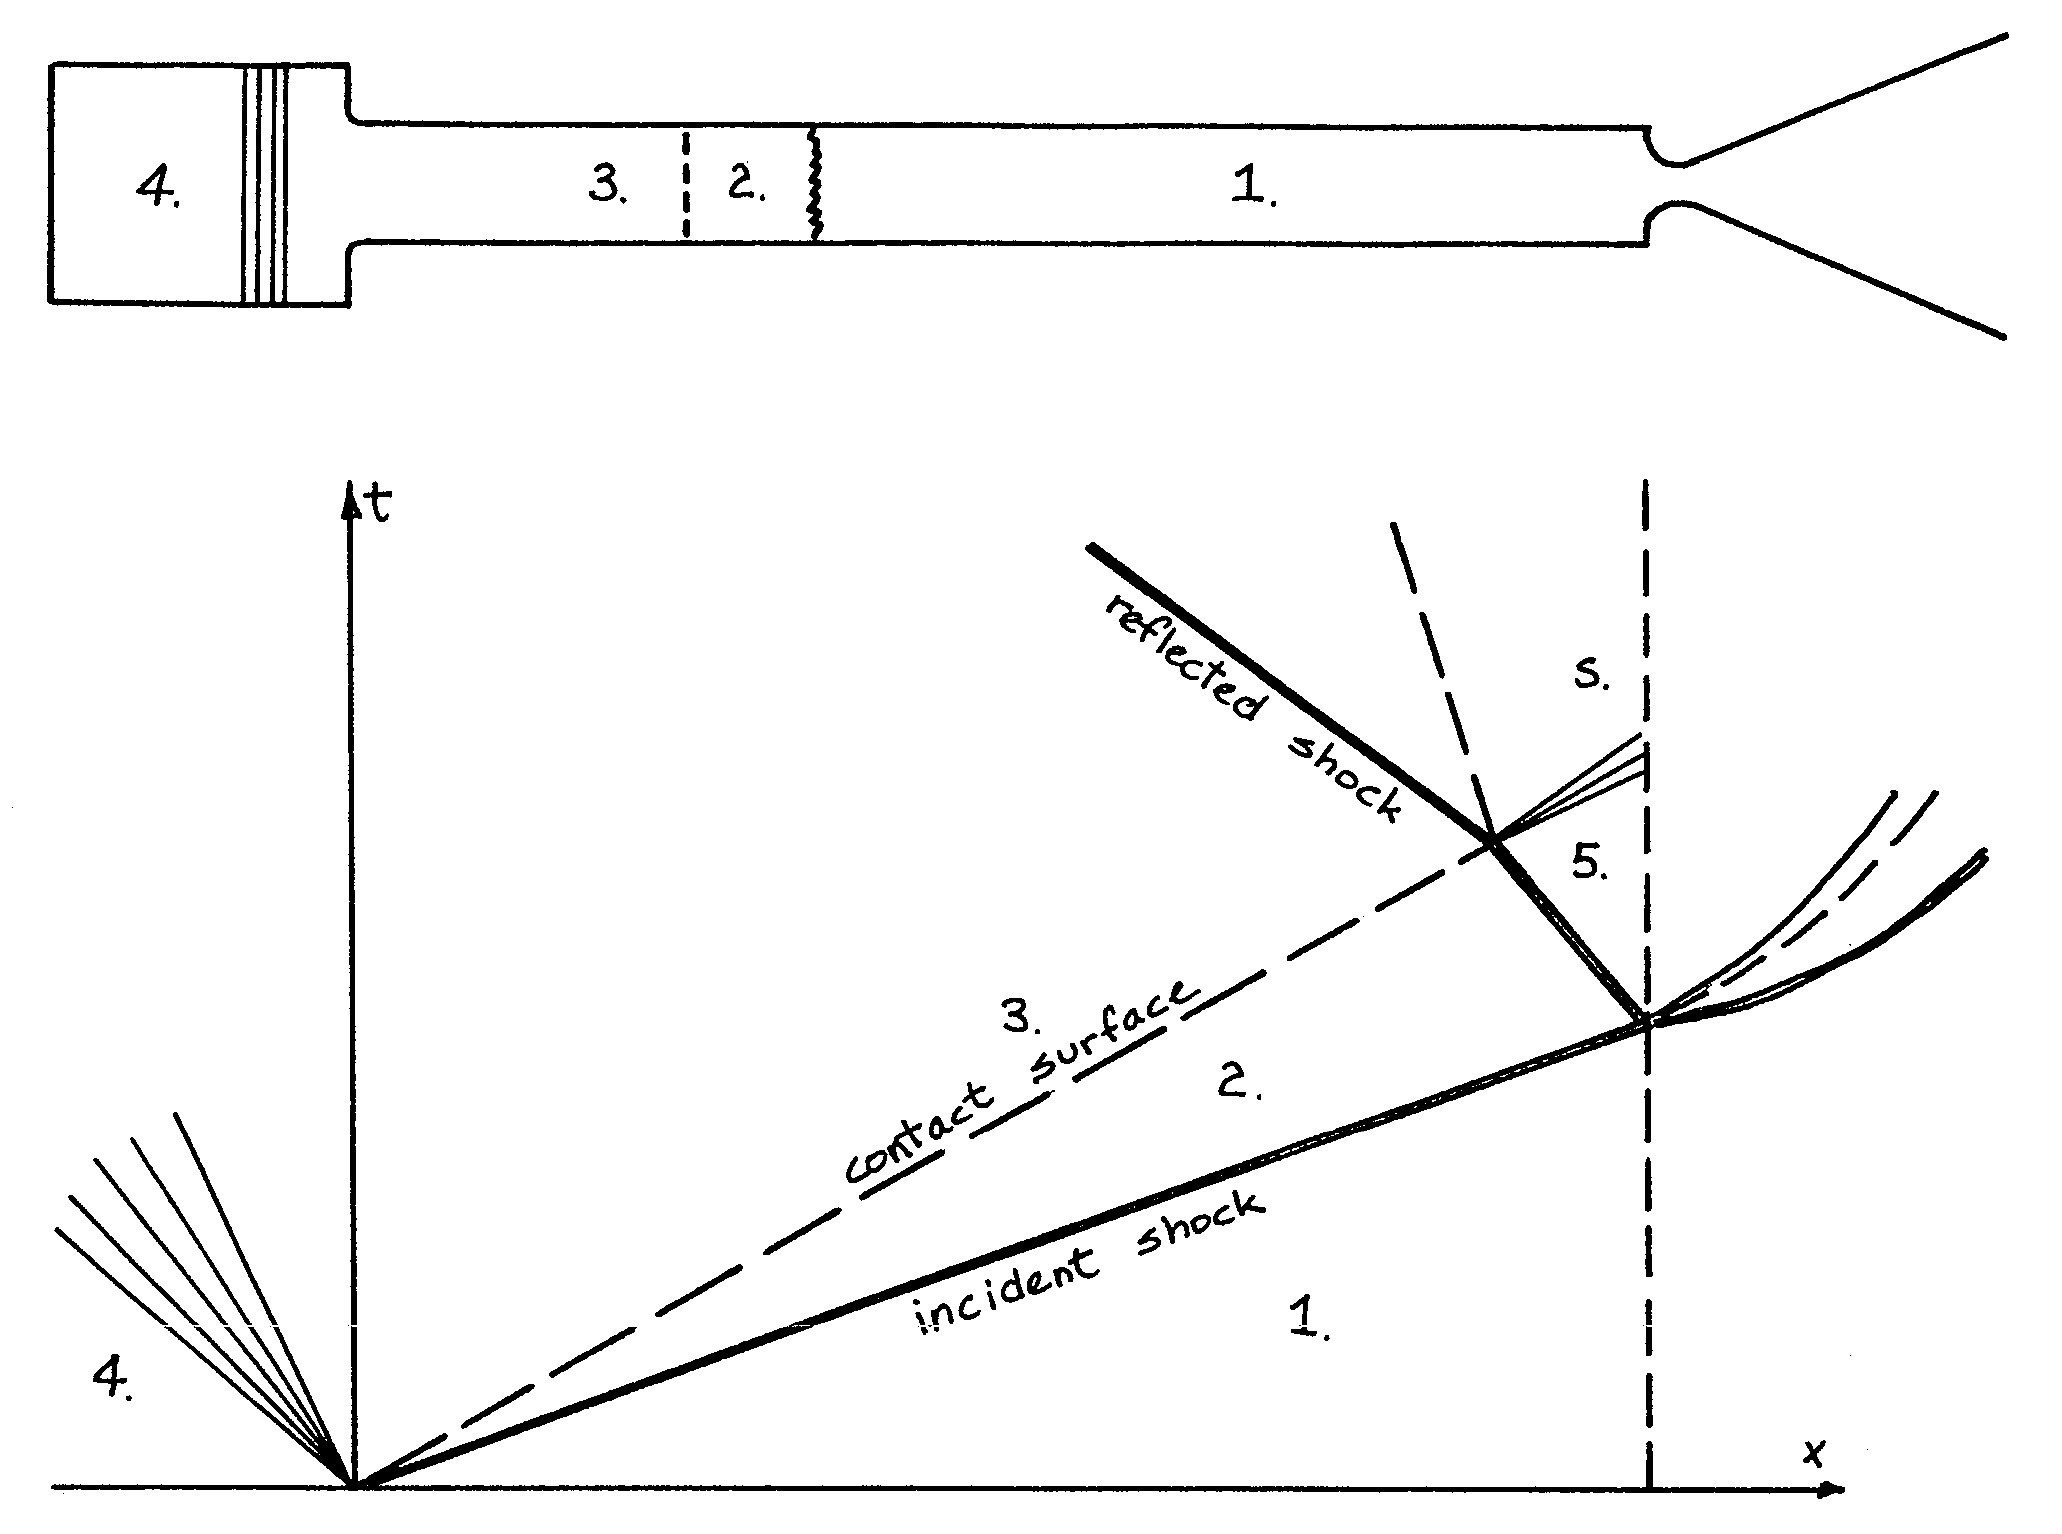
\includegraphics[width=0.7\textwidth]{../figs/shock-tube-process-fig-from-stn-report.png}
\end{center}

\medskip
A typical low-enthalpy flow condition for the T4 shock tunnel may start with
a test gas (air) at room temperature ($T_1$ = 300\,K) 
and a little above atmospheric pressure ($p_1$ = 125\,kPa).
The observed shock speed $V_s$ = 2414\,m/s and the observed nozzle-supply pressure
relaxed to 34.37\,MPa.
With the Mach 4 nozzle having an area ratio of 27, the flow conditions in the facility
may be computed using the command:
\begin{verbatim}
$ estcj.py --task=stn --gas=air --T1=300 --p1=125.0e3 --Vs=2414 --pe=34.37e6 --ar=27.0
\end{verbatim}
The full output is included below, where you should see that
this condition has an enthalpy of ($H_{5a} - H_1)$~=~5.43\,MJ/kg and the nozzle-exit condition
has a pressure of $P_7$~=~93.6\,kPa and a static temperature of $T_7$~=~1284\,K,
with a flow speed of $V_7$ = 2.95\,km/s.
Note that we have selected to stop the expansion at a particular nozzle area ratio.
Alternatively, we may stop the expansion at a particular Pitot pressure by specifying
\verb?--task=stnp? and a suitable ratio for the option \verb?--pp_on_pe?.
If you don't want to specify a relaxation pressure with option \verb?--pe?,
the reflected-shock conditions (5) will be used directly as the nozzle supply conditions.

\medskip
\noindent\topbar
\lstinputlisting[language={},breaklines=true]{../notes/t4-condition-transcript.txt}
\bottombar

\medskip
Subset calculations can be done by selecting a different task.
For example, just the incident shock processing can be computed with the \verb?--task=ishock?,
specifying only the gas, initial pressure, temperature and incident shock speed.

\medskip
The following sections show the subproblems that can be exercised from the command line.
These calculations can also be done inside other programs by calling 
the relevant \verb?gas_flow.py? functions.

\bigskip
\subsection{Pitot pressure calculation}
%
Using the test flow conditions from the exit of the Mach 4 nozzle, we can then
compute the expected Pitot pressure to be 2.14\,MPa.

\medskip
\noindent\topbar
\lstinputlisting[language={},breaklines=true]{../notes/pitot-transcript.txt}
\bottombar

\bigskip
\subsection{Cone surface pressure calculation}
%
Alternatively, the conditions on the surface of a conical pressure probe
(with 15$^o$ half-angle) can be computed as:

\medskip
\noindent\topbar
\lstinputlisting[language={},breaklines=true]{../notes/cone-transcript.txt}
\bottombar

\bigskip
\subsection{Total condition calculation}
%
The hypothetical stagnation conditions for a specified free stream
can be computed as:

\medskip
\noindent\topbar
\lstinputlisting[language={},breaklines=true]{../notes/total-transcript.txt}
\bottombar

\newpage
\section{The supporting libraries}
\label{the-libraries}
%
Although the ESTCj is built specifically to do the calculations 
needed for flow conditions typical of the T4 reflected shock tunnel,
the supporting libraries are more general.
There are gas modules for:
\begin{itemize}
 \item a perfect gas, with user specified properties (Appendix\,\ref{ideal-gas-py}).
 \item a mixture of gases in thermochemical equilibrium (Appendix\,\ref{cea2-gas-py}).
   This module delegates calculation to the CEA2 code.
 \item the same gas models that are used in the L1d3 and Eilmer3 codes,
   but with chemical reactions omitted (Appendix\,\ref{libgas-gas-py}).
\end{itemize}
%
The flow process modules cover the simple processes associated with:
\begin{itemize}
 \item normal shocks for one-dimensional flow.
 \item finite (isentropic) waves for one-dimensional flow.
 \item steady quasi-one-dimensional flow with area change.
 \item oblique shocks for planar and conical flow.
\end{itemize}
There is a module (Appendix\,\ref{gas-flow-py}) that uses 
the gas modules mentioned in the previous paragraph
and another (Appendix\,\ref{ideal-gas-flow-py})
that assumes a perfect gas model such that user needs specify the
relevant gas properties (such as the ratio of specific heats).

\medskip
This section is deliberately terse because the code in the appendices is well documented
and follows the standard texts on gas dynamics.
The only unusual formulation is that for the Taylor-Maccoll flow with the general gas model.
For that formulation, the notes from PJ's workbook are included 
in Appendix\,\ref{pj-notes-cone-flow}.


\bigskip
\subsection{Building custom application programs}
\label{custom-apps}
%
\subsubsection*{Classic shock tube}
%
As an example of building a custom application, consider the idealized shock tube 
with equal area sections separated by a diaphragm.
See for example, Section 7.8 (Shock tube relations) in Anderson's text\,\cite{anderson_82}
for a discussion based on perfect gas behaviour.

\medskip
\noindent\topbar
\lstinputlisting[language={}]{../../../eilmer3/2D/classic-shock-tube/classic_shock_tube.py}
\bottombar

\bigskip
\subsubsection*{Idealized expansion tube}
%
As a second example of building a custom application, consider the idealized expansion
of the test gas in an expansion tube\,\cite{trimpi_62}.
We will include just the processing of the test gas by the incident shock,
followed by the unsteady expansion to test-section conditions. 
The final expansion process is regulated by the fill pressure of the acceleration tube
and the test-gas conditions are determined by balancing the expanded gas pressure against
the post shock pressure of the acceleration gas.

\medskip
\noindent\topbar
\lstinputlisting[language={}]{../../../../lib/cfpylib/gasdyn/classic_expansion_tube.py}
\bottombar

%------------------------------------------------------------------

\newpage
\bibliographystyle{unsrt}
\bibliography{../bibtex/pj,../bibtex/shocktube,../bibtex/gas,../bibtex/gas_dynamic.bib}

%--------------------------------------------------------------------
% Appendices
%--------------------------------------------------------------------

\newpage
\appendix
\section{Source code for gas models}
%
\subsection{ideal\_gas.py}
\label{ideal-gas-py}
%
Thermodynamic functions for an ideal gas.

\noindent\topbar
\lstinputlisting[language={}]{../../../../lib/cfpylib/gasdyn/ideal_gas.py}
\bottombar

\newpage
\subsection{libgas\_gas.py}
\label{libgas-gas-py}
%
Thermodynamic functions for the gas model used by Eilmer3.

\noindent\topbar
\lstinputlisting[language={}]{../../../../lib/cfpylib/gasdyn/libgas_gas.py}
\bottombar

\newpage
\subsection{cea2\_gas.py}
\label{cea2-gas-py}
%
Thermodynamic functions for the thermochemical-equilibrium gas model backed by CEA2.

\noindent\topbar
\lstinputlisting[language={}]{../../../../lib/cfpylib/gasdyn/cea2_gas.py}
\bottombar

\newpage
\section{Source code for flow process calculations}
%
\subsection{ideal\_gas\_flow.py}
\label{ideal-gas-flow-py}
%
Basic flow relations for an ideal gas.

\noindent\topbar
\lstinputlisting[language={}]{../../../../lib/cfpylib/gasdyn/ideal_gas_flow.py}
\bottombar

\newpage
\subsection{gas\_flow.py}
\label{gas-flow-py}
%
Basic flow relations for a more general gas.

\noindent\topbar
\lstinputlisting[language={}]{../../../../lib/cfpylib/gasdyn/gas_flow.py}
\bottombar

\newpage
\section{Source code for ESTCj application}
\label{estcj-py}
%
Top-level application code.

\noindent\topbar
\lstinputlisting[language={}]{../../../../app/nenzfr/estcj.py}
\bottombar

\newpage
\section{Notes on conical flow}
\label{pj-notes-cone-flow}
%
Scanned straight from PJ's workbook, warts and all.

\begin{center}
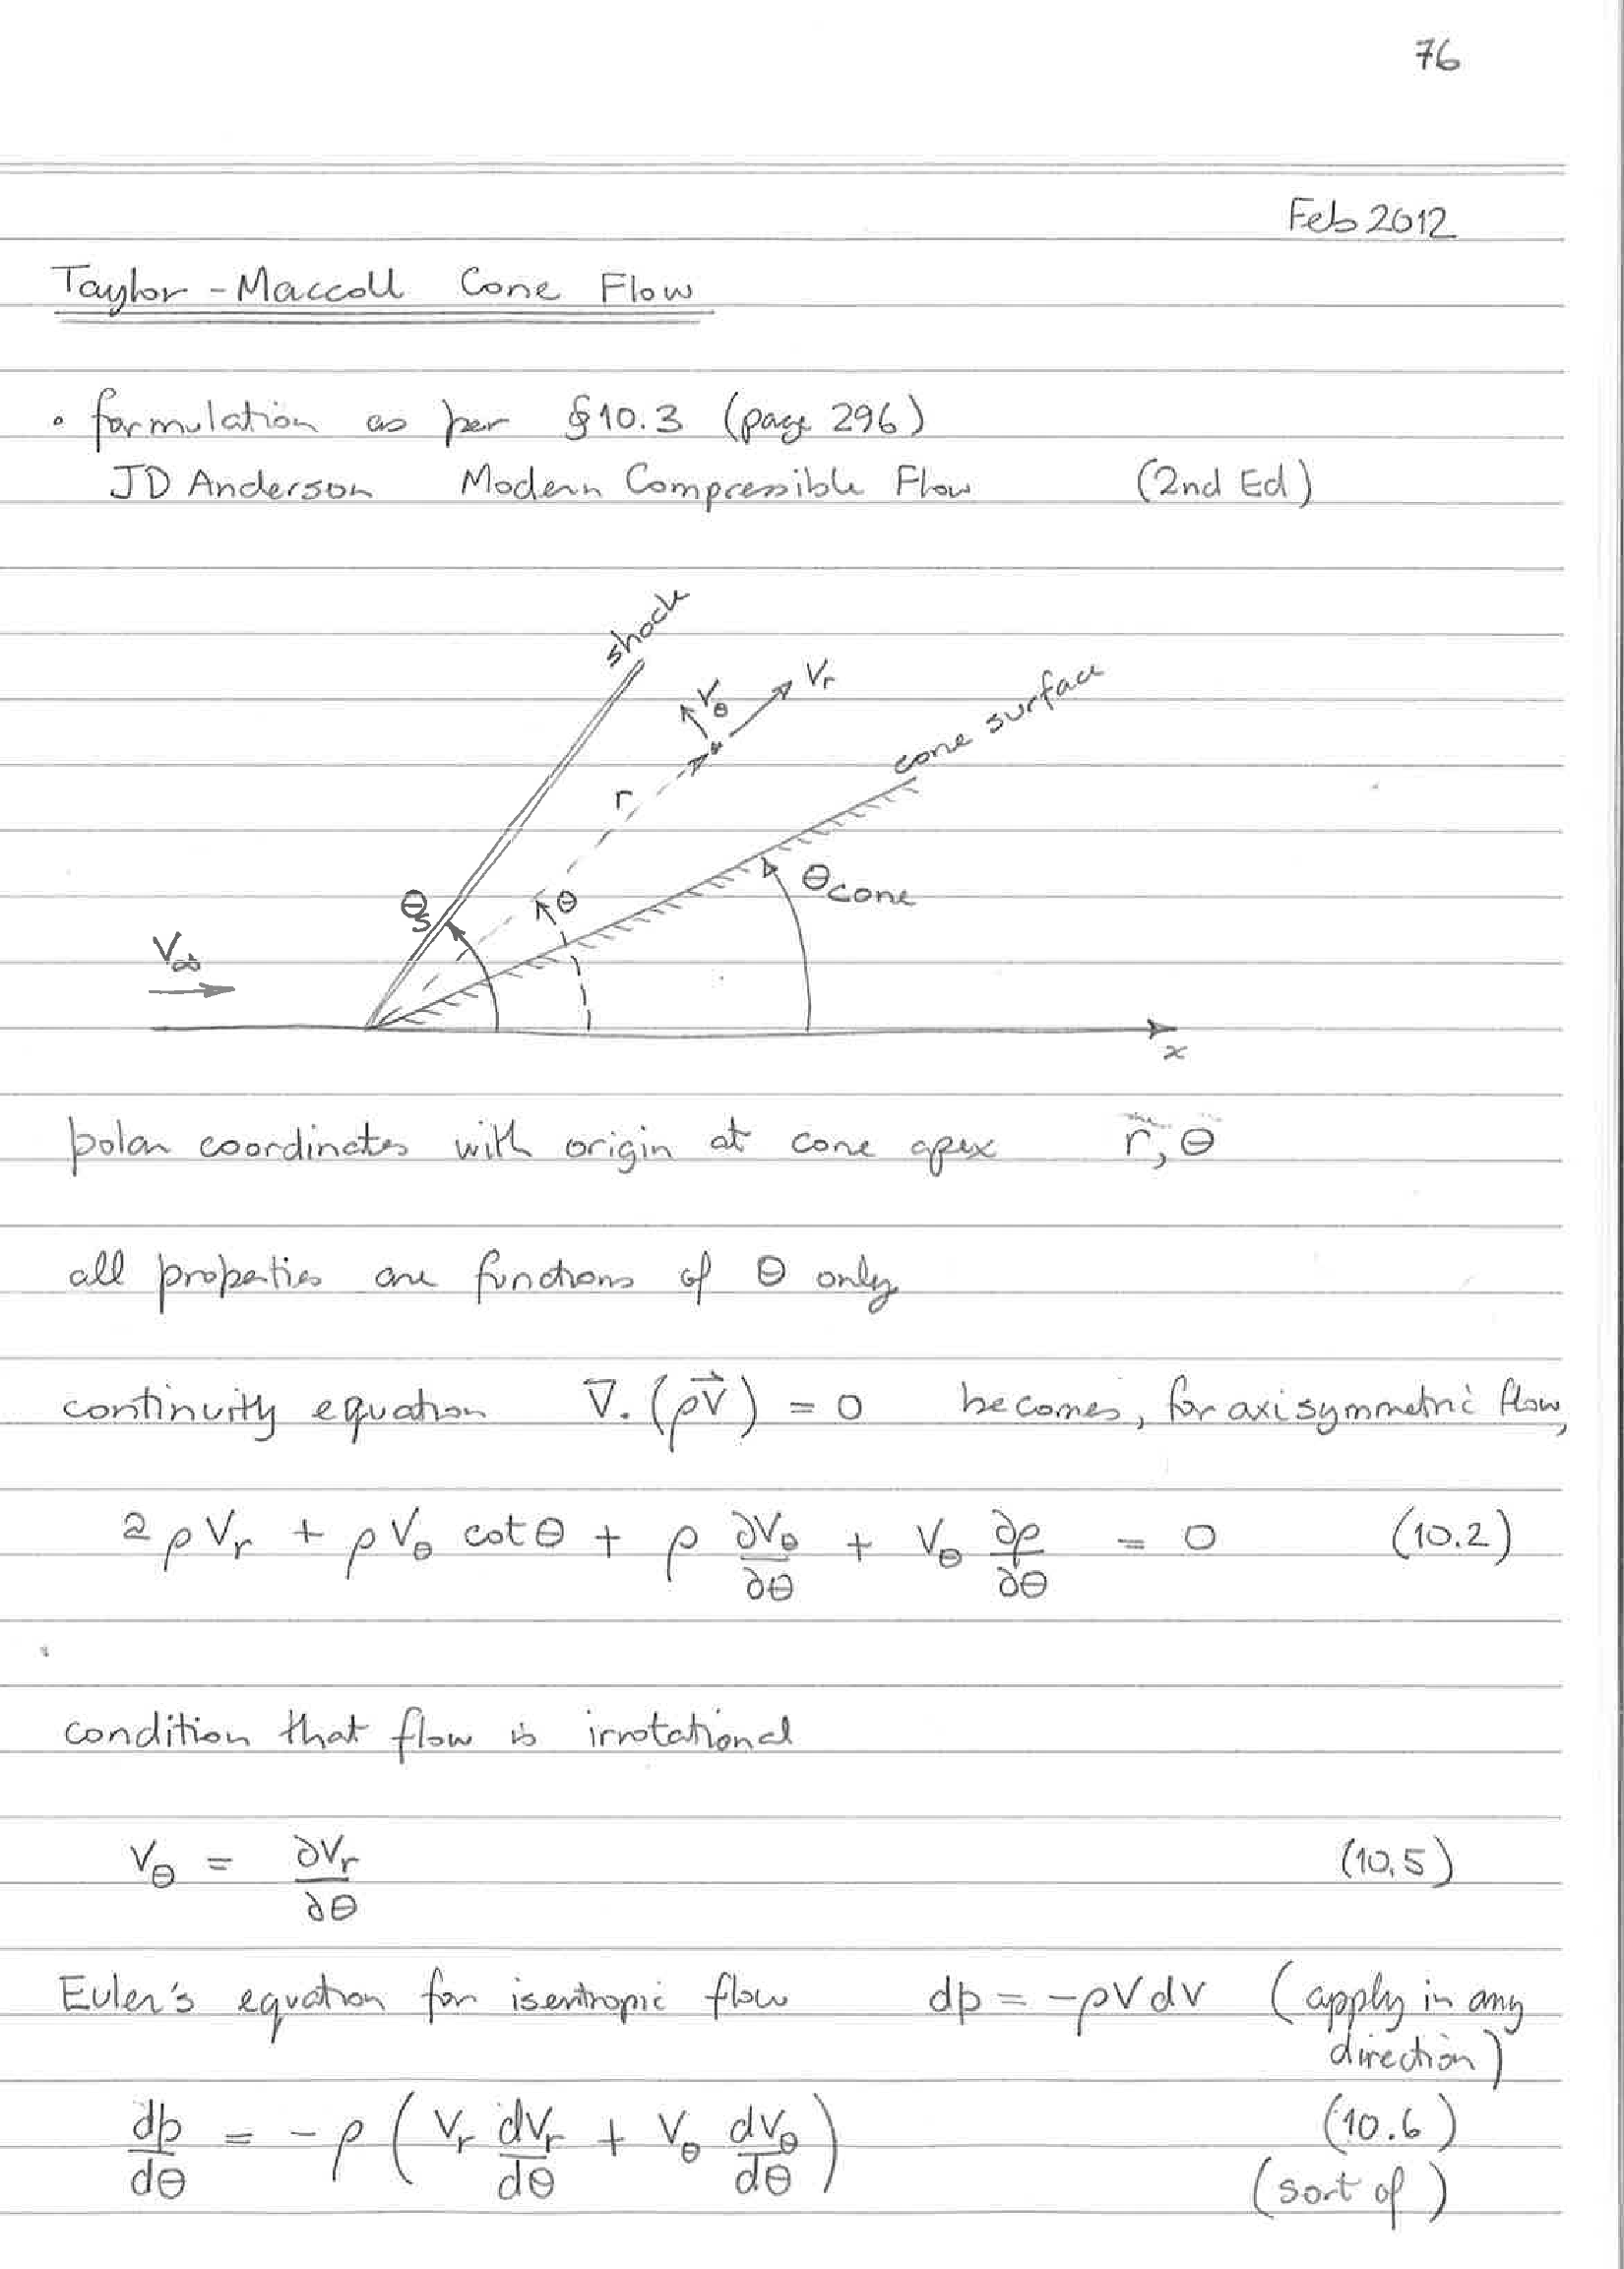
\includegraphics[width=\textwidth]{../figs/pj-workbook-page-76.png}
\end{center}

\newpage
\begin{center}
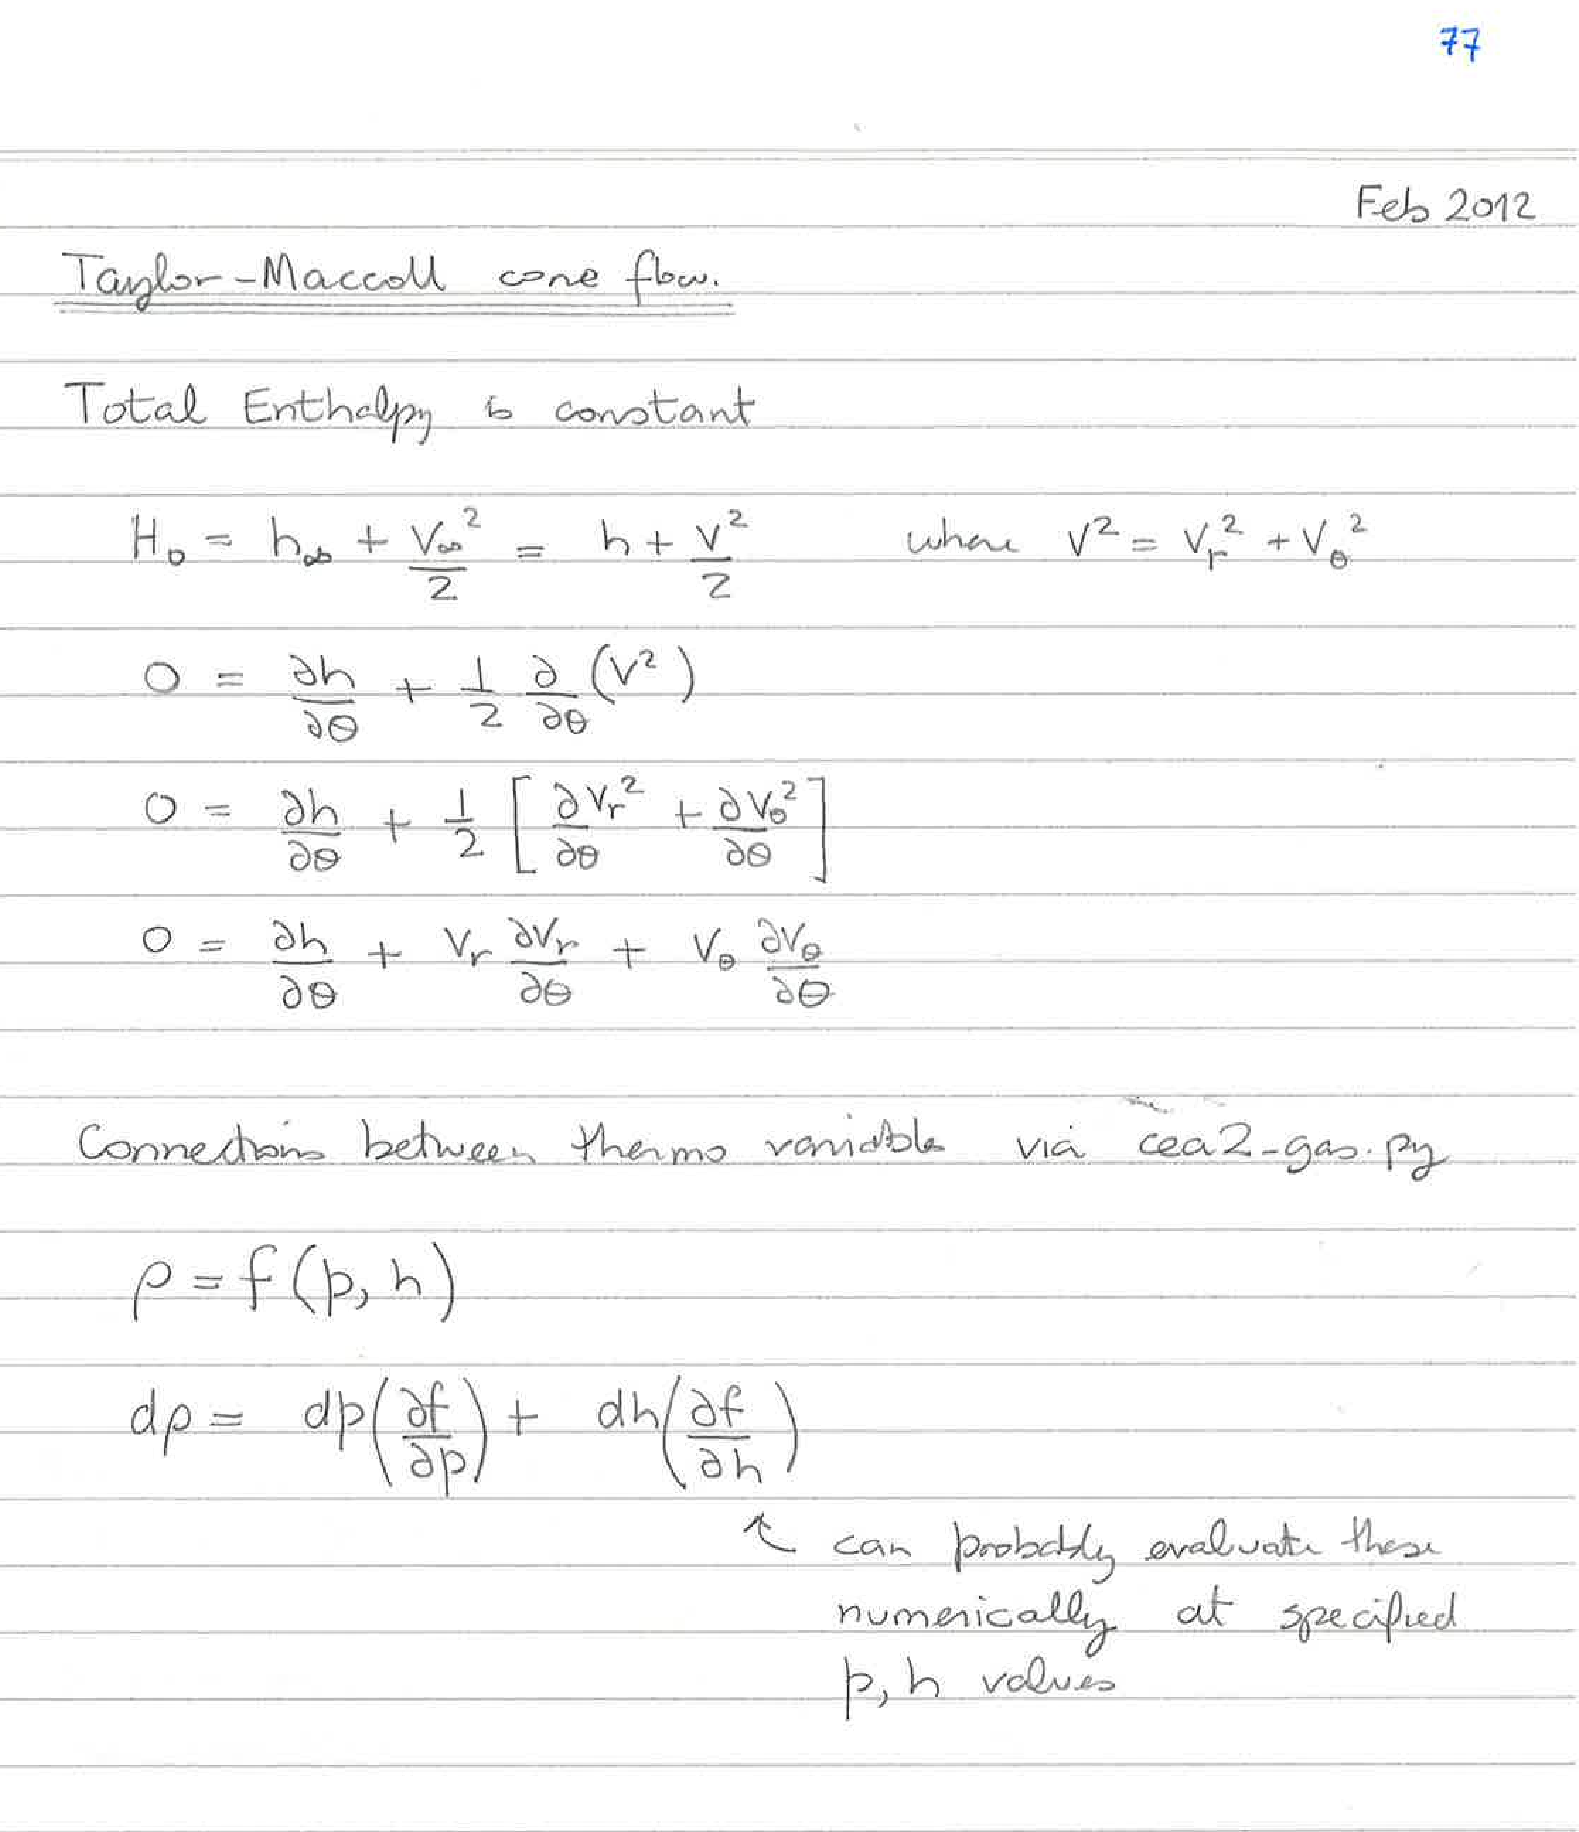
\includegraphics[width=\textwidth]{../figs/pj-workbook-page-77.png}
\end{center}

\newpage
\begin{center}
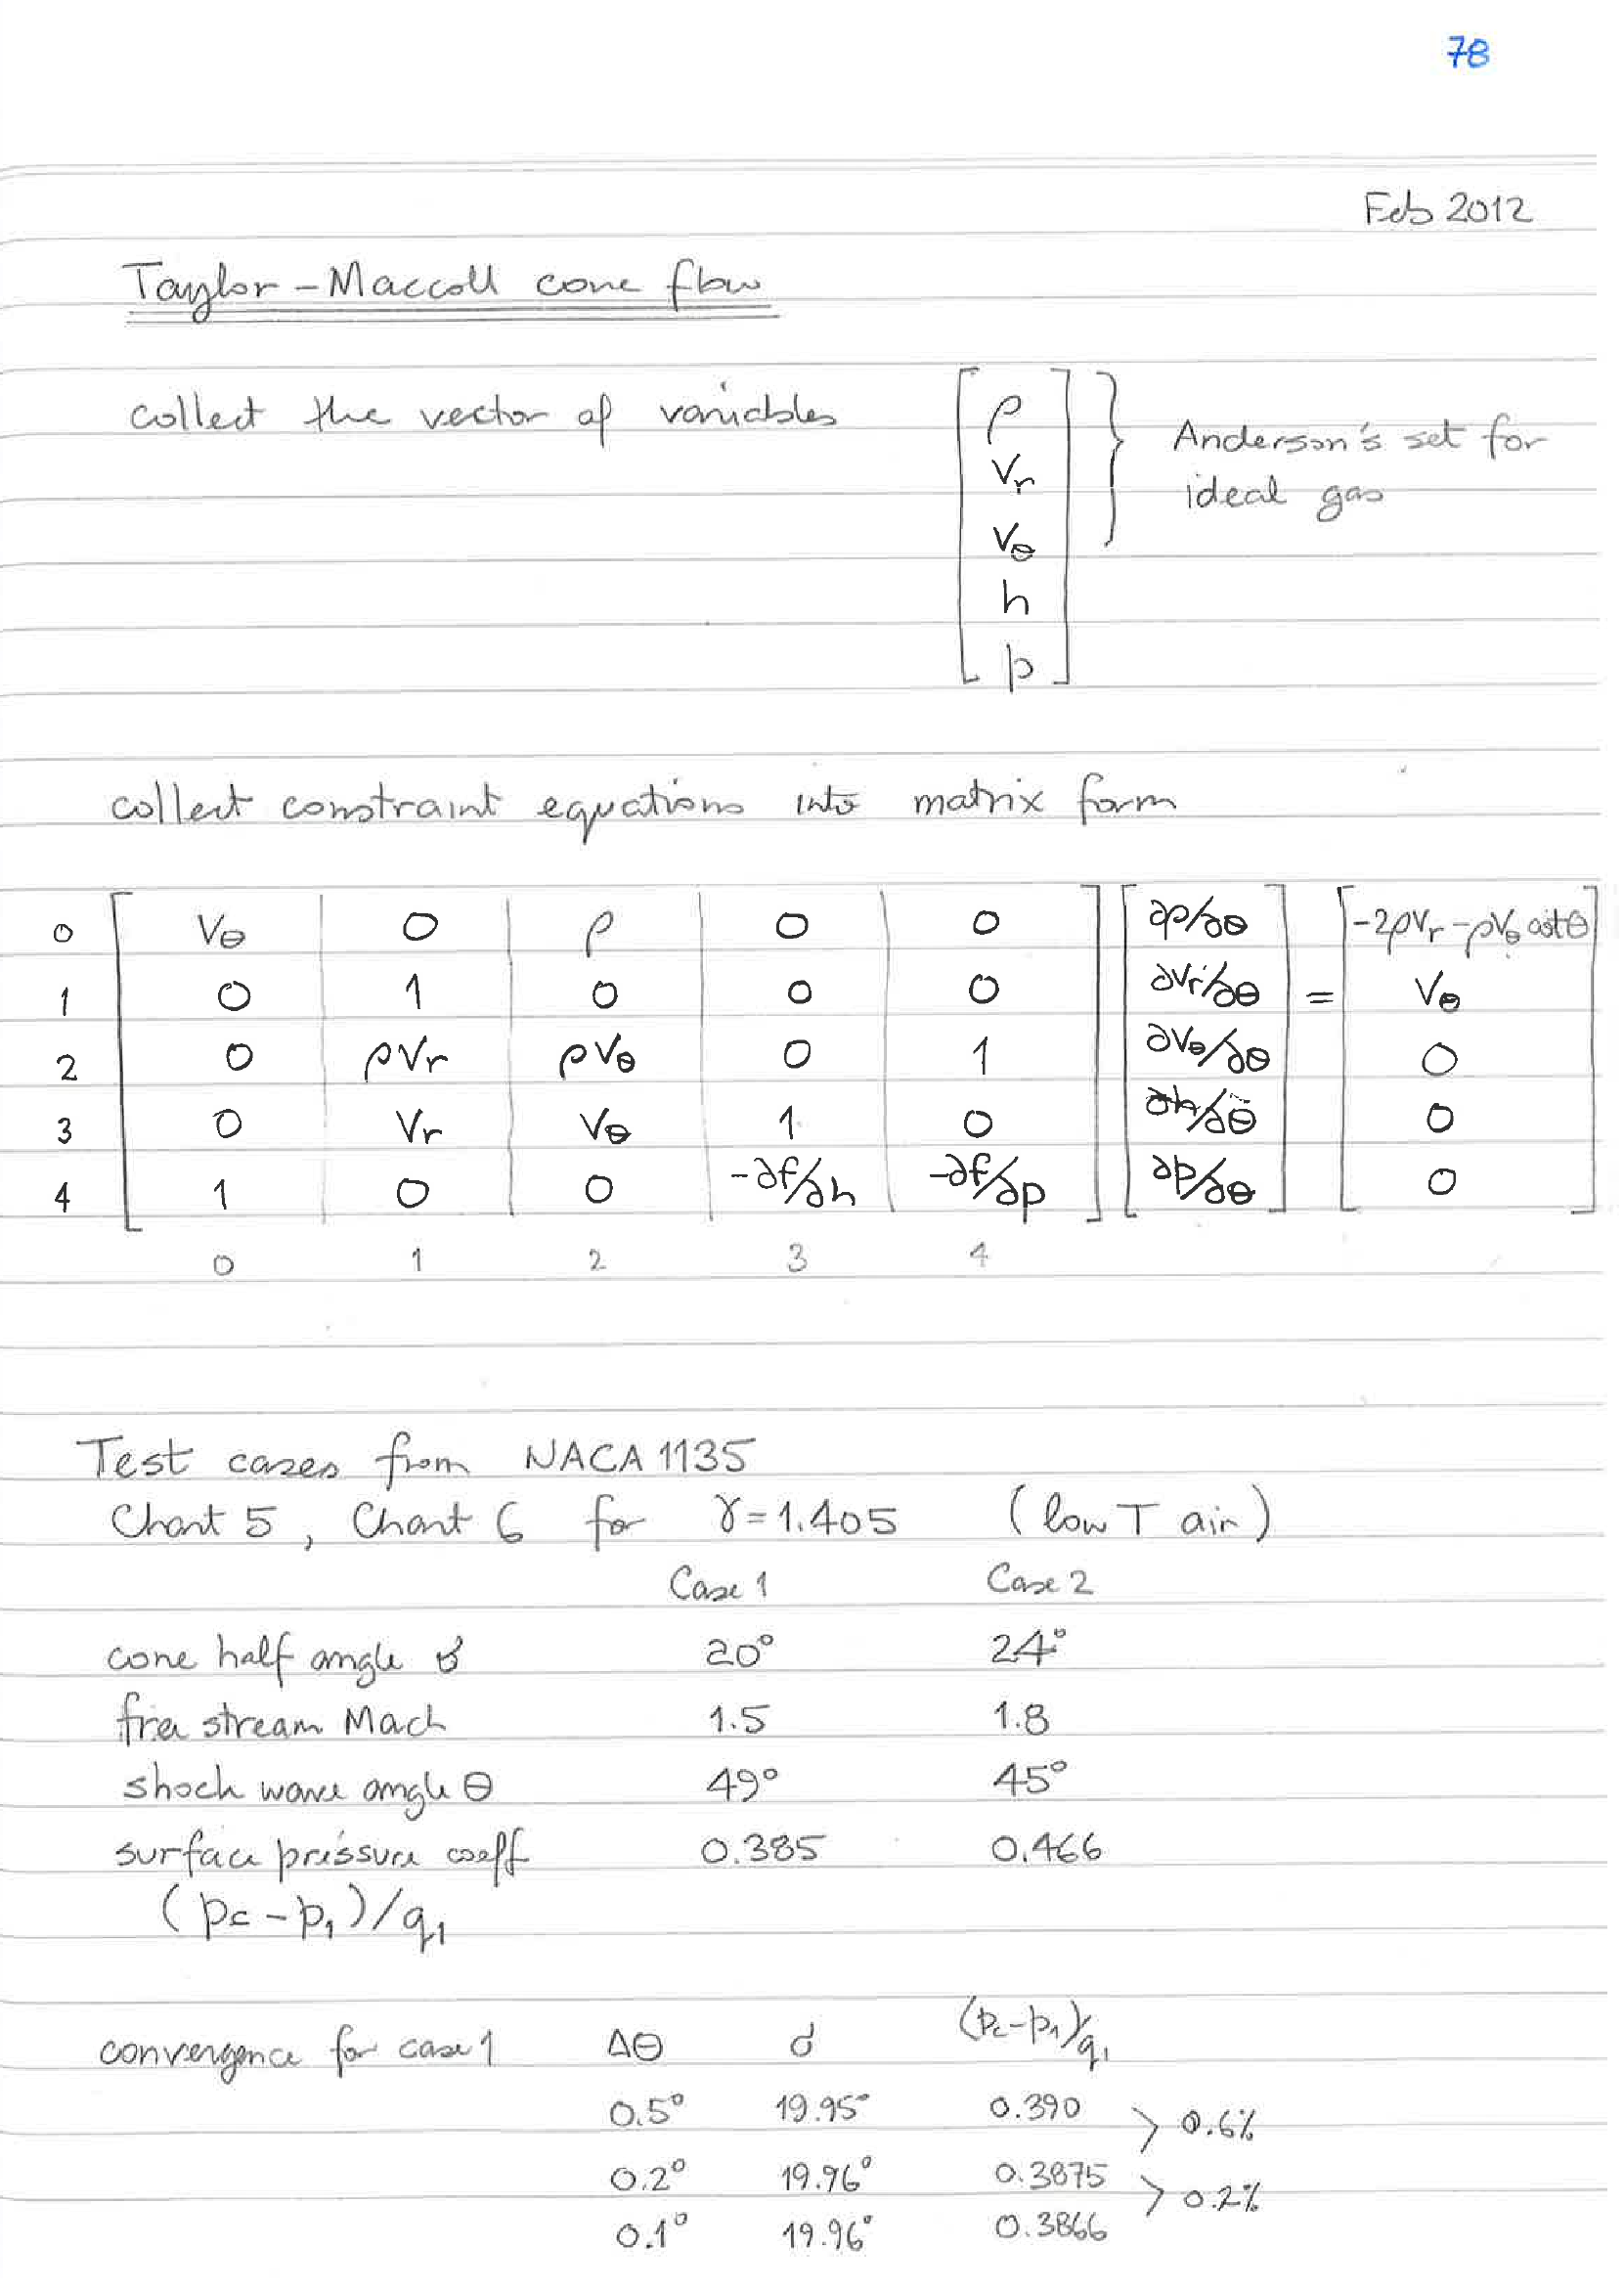
\includegraphics[width=\textwidth]{../figs/pj-workbook-page-78.png}
\end{center}

\end{document}

